%%%%%%%%%%%%%%%%%%%%%%%%%%%%%%%%%%%%%%%%%%%%%%%%%%%%%%%%%%%%%%%%%%
%%%%%%%% ICML 2010 EXAMPLE LATEX SUBMISSION FILE %%%%%%%%%%%%%%%%%
%%%%%%%%%%%%%%%%%%%%%%%%%%%%%%%%%%%%%%%%%%%%%%%%%%%%%%%%%%%%%%%%%%

% Use the following line _only_ if you're still using LaTeX 2.09.
%\documentstyle[icml2010,epsf,natbib]{article}
% If you rely on Latex2e packages, like most moden people use this:
\documentclass{article}

% For figures
\usepackage{graphicx} % more modern
%\usepackage{epsfig} % less modern
\usepackage{subfigure} 

% For citations
\usepackage{natbib}

% For algorithms
\usepackage{algorithm}
\usepackage{algorithmic}

% As of 2010, we use the hyperref package to produce hyperlinks in the
% resulting PDF.  If this breaks your system, please commend out the
% following usepackage line and replace \usepackage{icml2010} with
% \usepackage[nohyperref]{icml2010} above.
\usepackage{hyperref}

% Packages hyperref and algorithmic misbehave sometimes.  We can fix
% this with the following command.
\newcommand{\theHalgorithm}{\arabic{algorithm}}

% Employ the following version of the ``usepackage'' statement for
% submitting the draft version of the paper for review.  This will set
% the note in the first column to ``Under review.  Do not distribute.''
\usepackage{icml2010} 

% Employ this version of the ``usepackage'' statement after the paper has
% been accepted, when creating the final version.  This will set the
% note in the first column to ``Appearing in''
% \usepackage[accepted]{icml2010}

\newcommand{\F}{\mathcal{F}}
\newcommand{\PY}{\mathcal{P}\mathcal{Y}}
\newcommand{\G}{\mathcal{G}}
\newcommand{\ES}{\mathcal{E}\mathcal{S}}
\newcommand{\DP}{\mathcal{D}\mathcal{P}}

% The \icmltitle you define below is probably too long as a header.
% Therefore, a short form for the running title is supplied here:
\icmltitlerunning{Forgetting Counts}

\begin{document} 

\twocolumn[
\icmltitle{Constant Memory Inference \\
for Discrete Dependent Hierarchical Pitman-Yor Processes}

% It is OKAY to include author information, even for blind
% submissions: the style file will automatically remove it for you
% unless you've provided the [accepted] option to the icml2010
% package.
\icmlauthor{Nicholas Bartlett}{bartlett@stat.columbia.edu}
\icmladdress{Columbia University,
Room 1005 SSW, MC 4690,
1255 Amsterdam Avenue, New York, NY 10027}

\icmlauthor{Frank Wood}{fwood@stat.columbia.edu}
\icmladdress{Columbia University,
Room 1005 SSW, MC 4690,
1255 Amsterdam Avenue, New York, NY 10027}

% You may provide any keywords that you 
% find helpful for describing your paper; these are used to populate 
% the "keywords" metadata in the PDF but will not be shown in the document
\icmlkeywords{compression Pitman-Yor memory}

\vskip 0.3in
]

\begin{abstract} 
We propose a hierarchical Bayesian nonparametric model for discrete data that can be represented in constant space and estimated incrementally in linear time.  The inference procedure can be viewed as either approximating a model whose complexity grows as a function of the data or as estimation of a sequence of dependent nonparametric distributions.  We devise two estimation schemes corresponding to the two interpretations, a random deletion scheme and a greedy deletion scheme.  When tested on general compression corpora both procedures approach the performance of linear space methods while using significantly less memory, as well as outperforming both finite-depth models with the same memory bounds and standard compression methods.
\end{abstract} 

\section{Introduction}
\comment{
Nonparametric models, Bayesian or not, are characterized by computational and memory complexity that grows as a function of the size of the training data.  Unfortunately in common practice the relationship between training dataset size and complexity is used to select a dataset whose size is sufficiently small to allow model estimation.  Clearly this is not ideal given a sufficiently large and complex dataset.

When the computer is fixed but the dataset is not of fixed size but instead grows monotonically, two constraints are imposed on the computational complexity of inference and estimation procedures.  First, the computational complexity of estimation and inference cannot be greater than linear in the size of the data.  Second, the memory complexity of such algorithms must be constant.  Also, particularly in the case of growing data, the only suitable estimation and inference procedures are those that are incremental in nature.
}
In this paper we define a  (time-)dependent hierarchical Pitman-Yor process (HPYP) \cite{Teh2006a} and develop a {\em constant space, linear time} incremental inference procedure for models of discrete data based on it.   This contribution can be described as a ``forgetting'' procedure for existing HPYP inference procedures that retains only a ``good,'' constant-sized subset of the training data.  In designing and justifying such a model and inference procedure we extend methods for defining and doing inference in (time-)dependent sequences of Pitman Yor processes \cite{Caron2007, Caron2007a} to the hierarchical case.    We propose an incremental inference procedure for the resulting model that has two interpretations.  It can either be interpreted as either a valid inference procedure for a sequence of dependent HPYP's or as invalid (but approximately correct) inference procedure for a single non-varying HPYP.   In the latter case, our approach can be described as restricting the estimated model at all times  to the constant size model that ``best'' approximates (in some sense of the word best) a full model that would otherwise grow in the size of the training data.   

Previous work on dependent Dirichlet and Pitman-Yor processes \cite{MacEachern2000, Srebro2005, Griffin2006, Caron2007, Caron2007a} was motivated by the desire to construct generative procedures that induce dependence between related processes.  In our work we are motivated instead by the goal of performing constant space inference in a HPYP.  As the HPYP is a (Bayesian) nonparametric model, in order to achieve this we must ``forget'' data.  Conveniently, forgetting is one of the main mechanisms for generating (and performing inference) in models of sequences of dependent processes.  This hints at why our inference procedure can be interpreted in two ways.  If the true generative process varies in some dependent way, then it is possible that the implicit dependency induced by a forgetting procedure can capture and model that variation.  If, on the other hand, the true generative process is does not vary then, given our constant memory constraint on our (nonparametric) model, we still must forget.  This means choosing a  most informative subset of the data to retain and absorbing the risk of using an estimator that is possibly inconsistent.  This strategy of selecting a most informative subset of training data is not unique in the Bayesian nonparametric modeling literature.  In sparse Gaussian process modeling, forgetting strategies are used to achieve constant time and space (independent of the number of observations) inference procedures \cite{ Lawrence2003, Csat'o2002, Snelson2006}.

% in HPYP inference, namely efficient ways to identify and represent deep HPYP models \cite{Wood2009}, incremental inference techniques for the same \cite{Gasthaus2010}, and results from 
 
There is a very practical motivation for doing constant space inference in HPYP models.  A  {\em linear space, linear time} incremental estimator for the sequence memoizer (SM) \cite{Wood2009} (an HPYP model of unbounded depth for discrete sequence data) has been developed \cite{Gasthaus2010}.   A consequence of this development is that a SM could be deployed as the probabilistic sequence prediction model in a general purpose lossless compressor.   A compressor built in this way was shown to be better than other, general purpose lossless compressors (including gzip, bzip2, etc.).  Unfortunately the $O(n)$ memory complexity bound (where here $n$ is the length of the sequence) makes the SM impractical for use in a compressor.  Both very long sequences and arbitrarily long data streams cannot be modeled on a fixed computer and therefore cannot be compressed.  The obvious approach of estimating a new model for each of a number of constant size subsequences achieves the constant memory bound but, as we will show, can consistently be improved upon.   We show that our proposed constant space HPYP model and inference procedure achieves near optimal results for reasonable (practical to implement on modern computers) memory constraints.  This suggests that it might be possible to build and deploy an improved, practical, state-of-the-art compressor based on a constant space HPYP sequence prediction engine.

In the next section we review the Pitman-Yor process, the HPYP, and the 
SM.   Section~\ref{sec:theory} describes dependent Pitman-Yor processes and defines a dependent hierarchical Pitman-Yor process.   Section~\ref{inference} describes a sequential Monte Carlo inference procedure for the dependent hierarchical Pitman-Yor process defined in Section~\ref{sec:theory}.  Finally  Section~\ref{results} compares the predictive performance of the constant memory model to more complex models whose complexity is allowed to grow.  Why the predictive performance of the constant memory model is comparable to that of more complex models for reasonable memory bounds is discussed in Section~\ref{discussion}.

%If the memory complexity of the estimated model is constant with respect to training data size then both no more than a constant number of datapoints can be retained and no more than a constant number of parameters can be used.  It seems strange then to consider constant memory inference for a nonparametric model because, fundamentally, the resulting constant memory model estimate must be parametric.

%Regardless, the Gaussian process regression literature, for one example, includes many such approaches anyway \cite{gaussian process regression stuff, lawrence, csato, snelson, etc}.  The reason for this is that inference of Gaussian process regression models requires $O(n^2)$ space and $O(n^3)$ time where $n$ is the (growing) number of observations,  hindering their widespread use.  

%Inference in a simple (non-sparse) nonparametric kernel density estimator (assuming the kernel has broad support) requires access to all of the training data.  Large, fixed size datasets can often be accommodated by either engineering strategies (parallelism, etc.)~or approximation schemes (careful selection of representative subsets of the data).  Of course, fixed size data 

\comment{
%Bayesian nonparametric models interpolate between nonparametric 

%It can be difficult to distinguish between ``number of parameters,'' model ``complexity,'' and 


Parametric and nonparametric models differ in several key ways.  One important way is that parametric models have a fixed, finite number of parameters whereas nonparametric models are often described as having an effective number of ``parameters'' (often the datapoints or a subset of the datapoints themselves) that grows as a function of the size of the training data.

%An example of the former is Gaussian mixture model.  An example of the latter is a kernel density estimator.  In the former the number of mixture components is fixed a priori and the inference goal might be, in the case of density estimation, to find parameters that maximize the probability of the training data under the model.  In the latter, kernel density estimation case, the ``parameters'' of the model are the data points themselves (and perhaps parameters for a kernel function).  Here the effective number of parameters clearly grows linearly in the size of the training data. 

Bayesian nonparametric (BNP)  models are, somewhat confusingly, described as having ``complexity'' that grows as a function of the number of training data observations \cite{griffiths}.  BNP models are characterized by infinite dimensional parameter spaces \cite{sethurman, gaussian process function space reference}.   The former perspective derives from the fact that many BNP models can be ``collapsed'' in the sense that the infinite dimensional parameter space can be marginalized out yielding a simple, finite (for any finite dataset) representation whose memory complexity grows as a function of the training data size  (Chinese restaurant process \cite{CRP}, Polya urn representation \cite{poly urn}, etc.).  



%As a concrete example consider sequential importance sampling inference for a exponential family (conjugate) Dirichlet process mixture \cite{DP particle filter work}.  a fully collapsed representation can be used in which only the counts per class and sufficient statistics for each class need to be represented.


In such schemes, instead of representing the full infinite dimensional parameter space (or a truncation of it \cite{blei variational stuff}), such a collapsed representation instead only realizes and represents that part of the infinite dimensional parameter space ``responsible'' for generating the training data.     

%This difference in description is perhaps best explained through an example.  In a model with a Dirichlet process prior like $x_i | \G \sim \G, \G|\alpha,\G_0 \sim \DP(\alpha, \G_0),\; i=1\ldots n$,  either the posterior distribution of $\G |  \{x_i\}_{i=1}^{n},\alpha,\G_0$ or the posterior predictive distribution of $x_{n+1} | \{x_i\}_{i=1}^{n},\alpha,\G_0$ may be of interest.   In the former case, since it is known that both a priori and a posteriori that $\G$ has the form $\G = \sum_{k=1}^\infty \pi_k \delta_{\phi_k}$ \cite{sethurman} it is clear that the number of parameters in the model is infinite (there are an infinite number of so-called ``sticks,'' $\pi_k$ and ``atoms'' $\phi_k$).  On the other hand, ``marginal'' posterior predictive inference can be performed in such a model with $\G$ analytically integrated out.  Such inference utilizes representations in which the ``effective'' number of parameters in the model (really the state required to represent a single exact sample) grows in expectation as a function of the number of training data observations (Polya urn and Chinese restaurant process samplers \cite{plya_urn, crp} for example).  Other BNP models exhibit similar characteristics.

There is a connection between the effective number of parameters and the storage requirement for 

While nonparametric approaches (\cite{lots of shit}) in general, and BNP approaches in particular (\cite{lots more shit}) have exhibited empirical promise in a wide variety of application domains, enthusiasm for such methods should be damped by the realization that even sub-linear growth in the effective number of parameters is extremely problematic.  This is because, for any ``life-long'' learning agent, or any inference procedure exposed to extremely large training data sets, such growth will eventually make inference prohibitively expensive.  

In the BNP literature, this issue most acutely arises in Gaussian process (GP) models, where storage and computational complexity grow quadratically and cubically in the training data size.  To apply GP models to datasets of more than a few thousand data points requires using sparse variants that all effectively choose a ``best'' subset of the training data instances \cite{snelson, csato, etc}.  



How much memory must be used to represent such a model is highly dependent on the inference approach (approximate versus exact) and the representation used (one parameter per observation, one parameter per table and assignment to tables)

%(a Gaussian process is parameterized by mean and covariance {\em functions}, a Dirichlet process by a  

%``speak for themselves''


%The task of general file compression with an algorithm requiring constant space is of obvious practical value.  In any application there will be only a finite amount of memory available and many excellent compression algorithms become unfeasible when compressing large files.  In order to address this task directly an algorithm which allows a specified maximum memory allocation prior to running is needed.  In the case of compression through the use of probabilistic models, the algorithm should control the amount of memory required by adapting the complexity of the model in an appropriate manner to accommodate the stated memory bounds.

%Probabilistic models have been shown to perform extremely well when combined with an entropy encoder in compression algorithms.  These models work by predicting the next type in a sequence of types, most often bytes, which make up a file.  The better the model is, the more efficient the encoding scheme and the higher the compression ratio.  The model referred to as a stochastic memoizer for sequence data [wood] has recently been shown to outperform several other such models for general compression tasks [Gasthaus].  Unfortunately many of these byte level prediction algorithms require space on the order of the sequence length and thus become unrealistic for very large files.

%Even for models with theoretically constant memory requirements, such as n-gram models, the memory restriction cannot be pre-specified and the theoretical value is such a gross overestimate of the likely memory requirements it does not provide insight regarding the parameterization of the model at the start.  In section 1 of this paper we will review the stochastic memoizer for sequence data [wood].
}


\section{Background}
\label{basicModel}

\subsection{Pitman-Yor Process}

The Pitman-Yor process is a distribution over distributions which generalizes the Dirichlet process through the inclusion of a third parameter.  If $\G \sim \PY(d,c,\G_0)$ we say $\G$ is distributed according to a Pitman-Yor process with discount parameter $d$, concentration parameter $c$, and base measure $\G_0$. In the case that $d = 0$ the Pitman-Yor process reduces to the Dirichlet process \cite{Pitman1997}. 

It is often easier to work in a representation where the random distribution $\G$ is analytically marginalized out.  One way to draw a sample $\{ \theta_j \}_{j = 1}^N$ in this representation is to use a two step process.  

\begin{eqnarray*}
\G | d,c,\G_0 &\sim& \PY(d,c,\G_0)\\
\theta_i | \G &\sim& \G  \hspace{.5cm} i = 1 \dots N
\end{eqnarray*}

The first step produces a partition of the integer $N$ which follows the two parameter Ewen's sampling distribution ($\ES_N(d,c)$) \cite{Ewens1995}.  The second step assigns to each of the $K$ segments of the partition a parameter $\psi_k$ drawn independently from $\G_0$.  We set $\theta_j = \psi_k$ for all integers $j$ in segment $k$ of the partion \cite{Blackwell1973}.

Samples can be drawn from the Ewen's sampling distribution using the Chinese Restaurant Process (CRP).  Since the connection between the CRP and the Ewen's sampling distribution is essential to developments later in the paper we describe here the CRP in detail. We imagine a restaurant with a countably infinite number of tables, capable of seating a countably infinite number of customers.  The first customer in the CRP sits down at an empty table.  Customers $2 \dots N$ are seated sequentially by seating the $j$'th customer at a table drawn from the following distribution:

\begin{eqnarray*}
p(\textrm{occupied table}_i |\textrm{ previous}) &=& \frac{n_i - d}{j-1+ c}\\
p(\textrm{unoccupied table} | \textrm{ previous}) &=& \frac{t_{j-1}d +c}{j-1+c}
\end{eqnarray*}

where $n_i$ is the number of customers already sitting at table $i$, $t_{j-1}$ is the number of tables occupied by the first $j-1$ customers, and previous refers to the seating arrangement of the first $j-1$ customers.  The final seating arrangement in the restaurant defines a partition of the integer $N$ which follows the $\ES_N(d,c)$ distribution \cite{Pitman1995}.  To complete the process of generating a sample $\{ \theta_j \}_{j = 1}^N$ we must endow each occupied table in the restaurant with a parameter $\psi_k$ drawn independently from $\G_0$.  We set $\theta_j = \psi_k$ if customer $j$ is sitting at table $k$.


\subsection{Hierarchical Pitman-Yor Processes}

Recent research has produced a spate of new hierarchical models using the Pitman-Yor process \cite{Teh2006b} \cite{Teh2006a}.  An an example hierarchical Pitman-Yor process is 

\begin{eqnarray*}
\G_1|d_1, c_1, \G_0 &\sim& \PY(c_1,c_1,\G_0)\\
\G_2 | d_2, c_2, \G_1 &\sim& \PY(d_2,c_2, \G_1)\\
\theta_i | \G_2 &\sim& \G_2 \hspace{.5cm} i = 1\dots N.
\end{eqnarray*}

To obtain a sample from the hierarchical Pitman-Yor process it is again useful to work in a representation where $G_2$ and $G_1$ are analytically marginalized out. One way to generate samples in this representation is to recursively apply the algorithm for the single Pitman-Yor process.  To draw a sample $\{ \theta_j \}_{j = 1}^N$ we again need to produce a partition of the integer $N$ following the $\ES_N(d_2,c_2)$ distribution.  This can be achieved using the CRP and in Figure~\ref{figHPY} is represented by the restaurant corresponding to $\G_2$. We will denote the number of tables in the child restaurant as $K_2$.  Each of the $K_2$ tables must be endowed with a parameter $ \psi_{2k}$ drawn independently from $\G_1$.  Since $\G_1$ has been marginalized out we obtain $\{ \psi_{2k} \}_ {k = 1}^{K_2}$ by again using the procedure for the single Pitman-Yor process.  A partition from the $\ES_{K_2}(d_1,c_1)$ distribution is produced via the CRP represented in Figure~\ref{figHPY} by the restaurant corresponding to $\G_1$. We denote the number of tables in the parent restaurant as $K_1$.   Each of the $K_1$ tables must be endowed with a parameter $\{ \psi_{1k} \}_{ k = 1}^{K_1}$,  independently drawn from $\G_0$.  We set $\psi_{2k}  = \psi_{1m}$ if in the parent restaurant customer $k$ is sitting at table $m$ and we set $\theta_j = \psi_{2k}$ if in the child restaurant customer $j$ is sitting at table $k$.

\begin{figure}[t] 
	\begin{center}
		\label{figHPY}
		\scalebox{.25}{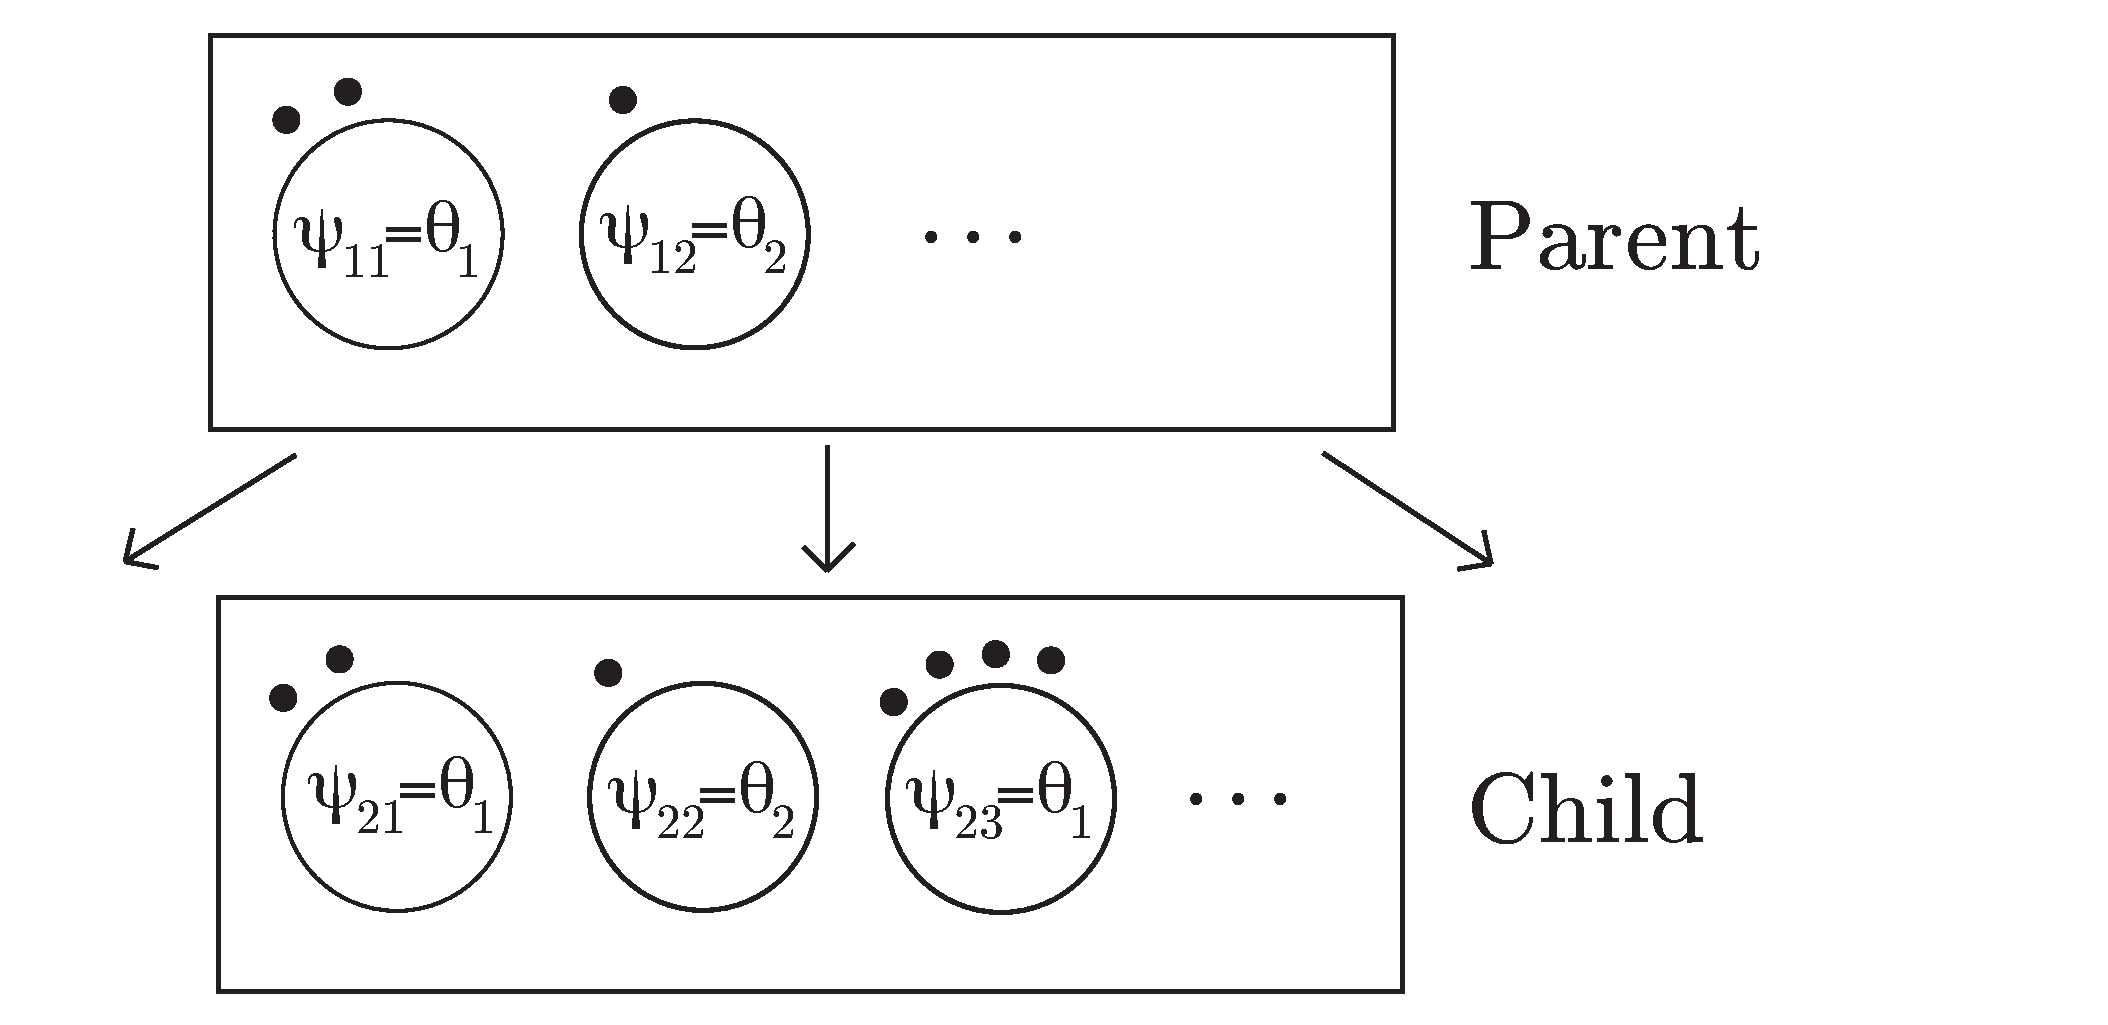
\includegraphics{figure1.pdf}} % [clip=true, viewport= 1in 1in 9in 9in]
		\caption{Final state of an example CRF process.}
	\end{center} 

\end{figure} 

An example is shown in Figure~\ref{figHPY} in which the CRP process for the child restaurant resulted in three tables ($K_2 = 3$).  Therefore, three parameters must have been drawn from $\G_1$.  Since $\G_1$ is marginalized out we again revert to the procedure for a single Pitman-Yor process. The CRP for the parent restaurant resulted in two tables ($K_1 = 2$).  $\psi_{11}$ and $\psi_{12}$ are drawn independently from the base distribution $\G_0$.  $\{ \psi_{2k} \}_{k = 1}^{K_1}$ is equal to $\{ \psi_{11}, \psi_{11}, \psi_{12} \}$ and finally  $\{ \theta_j \}_{j = 1}^7 = \{ \psi_{11}, \psi_{11}, \psi_{12},\psi_{11},\psi_{11}, \psi_{11}, \psi_{11}\}$.

The recursive application of the CRP in a hierarchical model is known as the Chinese restaurant franchise (CRF) \cite{Teh2006b}.  As alluded to in Figure~\ref{figHPY}, the number of child restaurants is not restricted to one.  Furthermore, the recursive nature of the CRF makes extensions to deeper hierarchies straightforward. For more more detail refer to \cite{Teh2006b, Teh2006a}.

\subsection{Sequence Memoizer}

The sequence memoizer (SM) \cite{Wood2009} is a model for discrete sequence data based on an unbounded depth hierarchical Pitman-Yor process. We can write the model as:

\begin{eqnarray*}
	\G_{[]} | \mathcal{U}_{\Sigma}, d_0 &\sim& \PY(d_0, 0, \mathcal{U}_{\Sigma }) \\
	\G_{\bf{u}} | \G_{\sigma(\bf{u})}, d_{|\bf{u}|} &\sim& \PY(d_{|\bf{u}|}, 0, \G_{\sigma(\bf{u})}) \hspace{.35cm} \forall \bf{u} \in \Sigma^+\\
	\theta_n | \theta_{n-1}  \ldots \theta_1 = \bf{u} &\sim& \G_{\bf{u}}
\end{eqnarray*}

where $\mathcal{U}_{\Sigma }$ is a uniform distribution over the set of symbols, $\bf{u}$ is a particular context, $\Sigma^+$ is the set of all such contexts, and $\sigma(\bf{u})$ is the context $\bf{u}$ modified by removing the most distant symbol.  We assume $| \Sigma | < \infty$. 

\begin{figure}[t] 
	\label{figprefixtree}
	\begin{center}
		\scalebox{.5}{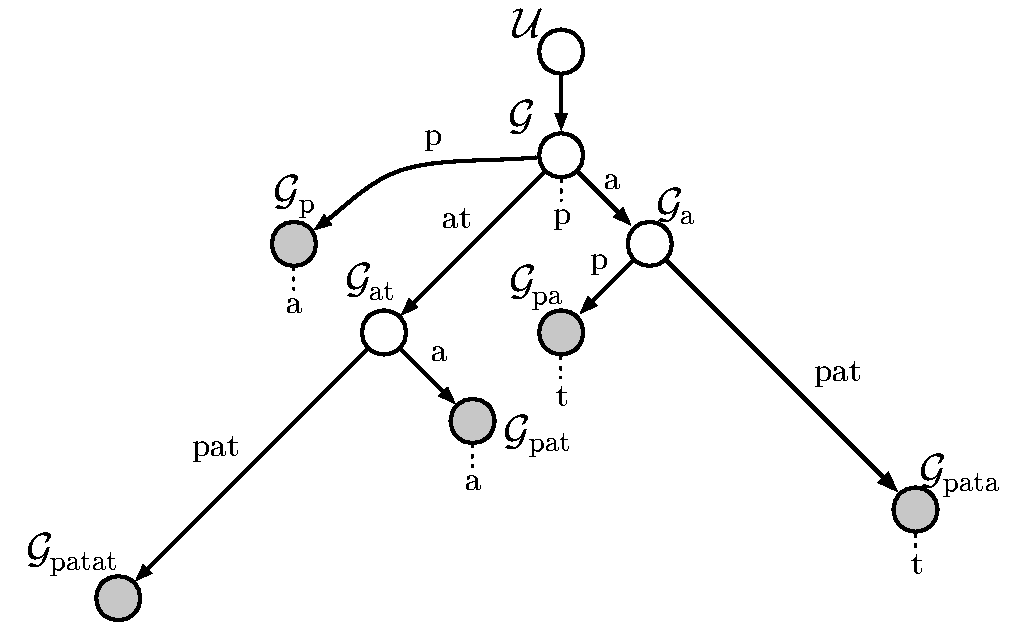
\includegraphics{prefix_tree.pdf}} % [clip=true, viewport= 1in 1in 9in 9in]
		\caption{An example prefix tree for the sequence $patat$}.
	\end{center} 
\end{figure} 

Figure~\ref{figprefixtree} shows the graphical model needed to to model the sequence $patat$.  Note that in the SM graphical model, nodes which are not branching nodes and are not associated with observed data are not instantiated.  This is because of an analytic result from \cite{pitman} showing that two Pitman-Yor processes can be analytically integrated against one another.  Note that this result is different than the result from \cite{mcqueen} allowing for the representation we are using which analytically integrates out each random distribution separately.  The node labeled $\G_{patat}$ is only shown in the graphical model to indicate that the next symbol in the sequence will come from this distribution.

Inference in the SM model is performed in the Chinese restaurant franchise respresentation. Inference takes worst case $\mathcal{O}(n^2)$ time and requires $\mathcal{O}(n)$ space where $n$ is the length of the sequence. Quadratic time stems from the fact that seating a customer in the appropriate restaurant may require seating a customer in all of the restaurants above it.  The length of this path is bounded by the length of the sequence. Each restaurant requires constant space because a restaurant need only maintain a constant number of summary statistics, the total number of customers and the total number of tables present of each type.\footnote{For symbol sets of finite cardinality.} Note this representation requires reinstantiation of the full restaurant state for some steps of inference which can be done by exploiting exchangeability.  The fact that a restaurant can be represented allows the full model to be represented in $\mathcal{O}(n)$ space.

In most applications $\mathcal{O}(n)$ space is acceptable, but for sequence modeling of extremely long sequences it is problematic.  Tasks such as compression often encounter sequences which make the SM an impractical option.  

\section{Theory}
\label{sec:theory}

While the SM model demonstrates promising empirical results \cite{Gasthaus} we are unsatisfied with the linear space requirement for reasons stated earlier.  We propose a framework for limiting the memory required to represent models based on the hierarchical Pitman-Yor process.  Estimation in this framework can be viewed either as a valid inference scheme for a model based on a dependent set of hierarchical Pitman-Yor processes or as an approximate inference technique for a non-varying model.

\subsection{Dependent Pitman-Yor process} 

The $\ES_N(d,c)$ distribution discussed in Section~\ref{basicModel} has an important consistency property. In the Chinese restaurant metaphor the consistency property corresponds to the fact that if a customer is removed uniformly at random, the remaining customer configuration represents a partition of the integer $N-1$ following the $\ES_{N-1}(d,c)$ distribution. Another deletion operation known as size-biased deletion, in which a customer is chosen uniformly at random and all customers seated at the same table are removed from the restaurant, is known to satisfy such a consistency property for the one parameter Ewen's distribution \cite{kingman}.  This is known as the species deletion property \cite{kingman}, but does not hold in the two parameter case \cite{pitman}

The consistency property allows the restaurant representation to be modified to draw samples  $\{ \theta_j^t \}_{i = 1}^{N_t}$ from a sequence of dependent random distributions $\{ \G^t \}_{t=1}^T$ such that 

\begin{eqnarray}
 \label{eqnDependentPY1}  \G^t | d, c, \G_0 &\sim& \PY(d,c,\G_0)\\
 \label{eqnDependentPY2}  \theta_j^t | \G^t &\sim& \G^t \hspace{.5cm} j = 1 \dots N_t.
 \end{eqnarray}
 
We use the index $t$ because of the useful interpretation as time even though it need not be a temporal sequence. The fact that $\G^t_1$ has the same distribution over time is known as stationarity \cite{davis and brockwel}.  
 
The generative procedure, an extension of the analogous procedure for dependent Dirichlet processes \cite{caron}, starts with an empty restaurant and generates $\{ \theta_j^1\}_{i = 1}^{N_1}$ by using the CRP to generate a partition of the integer $N_1$ and then endowing each table with a value drawn independently from $\G_0$.  Between time points customers are deleted uniformly at random from the customer configuration of the restaurant and empty tables are removed from the restaurant.  After the deletion step new customers are seated according to the CRP with the initial customer configuration of the process given by the configuration resulting from the deletion step.  Once new customers have been seated, previously unoccupied tables are endowed with a value drawn independently from $\G_0$.  We set $\theta^t_j = \psi_k$ if  the $j^{th}$ customer seated during the $t^{th}$ time step is seated at table $k$.

If $j$ customers are deleted after time step 1 the partition represented by the starting customer configuration of the restaurant at time step 2 follows a $\ES_{N_1- j}(d,c)$ distribution.  Therefore, after seating new customers in time step 2 the configuration results in partition which follows a $\ES_{N_1 - j + N_2}(d,c)$ distribution.  This is the only result needed to ensure Eqn.~\ref{eqnDependentPY1} and Eqn.~\ref{eqnDependentPY2}.  Note that the number of customers removed from the restaurant between time steps is independent of the consistency result and can thus be either stochastic or deterministic.

Dependence between $\G^t$ is induced by the modified restaurant representation through the undeleted customers.  An exact characterization of the dependence is non-trivial.   \cite{caron} show that in the analogous procedure for dependent Dirichlet distributions, removing fewer customers between time steps induces higher dependence.  In the extreme case of removing all the customers between time steps, the procedure generates samples drawn from independent $\G^t$. Removing no customers implies a $\G$ that is not varying with the index $t$. 

%TODO give graphical model
\subsection{Time-varying Pitman-Yor Process in a hierarchical setting}

Consider now the hierarchical dependent setting 

\begin{eqnarray*}
\G_1 | d_1, c_1, \G_0 &\sim& \PY(d_1, c_1, \G_0)\\
\G_2^t | d_2, c_2, \G_1&\sim& \PY(d_2, c_1, \G_1) \hspace{.5cm} t = 1\dots T\\
\theta^t_i | \G_2^t &\sim& \G_2^t \hspace{.5cm} i = 1\dots N_t.
\end{eqnarray*}

A generative procedure giving rise to data from this model is obtained by combining the Chinese restaurant franchise with the modified restaurant process.  The combination executed by removing customers, uniformly at random, from the restaurant corresponding to $\G_2$ between time steps.  The restaurant corresponding the $\G_1$ is unchanged between time steps. At each time, samples are drawn by first producing a partition from the Chinese restaurant franchise using initial restaurant configurations set to the restaurant configurations produced by the deletion step.  After seating the new customers,  previously unoccupied tables are endowed with a parameter $\psi_{2k}$ drawn independently from $\G_1$.  Since we are working in a representation with $\G_1$ analytically marginalized out $\psi_{2k}$ is drawn through the usual method using the CRP and the current customer configuration of the restaurant corresponding the $\G_1$.


\begin{figure}[h!tbp] 
	\label{figVHPY}
	\begin{center}
		\scalebox{.25}{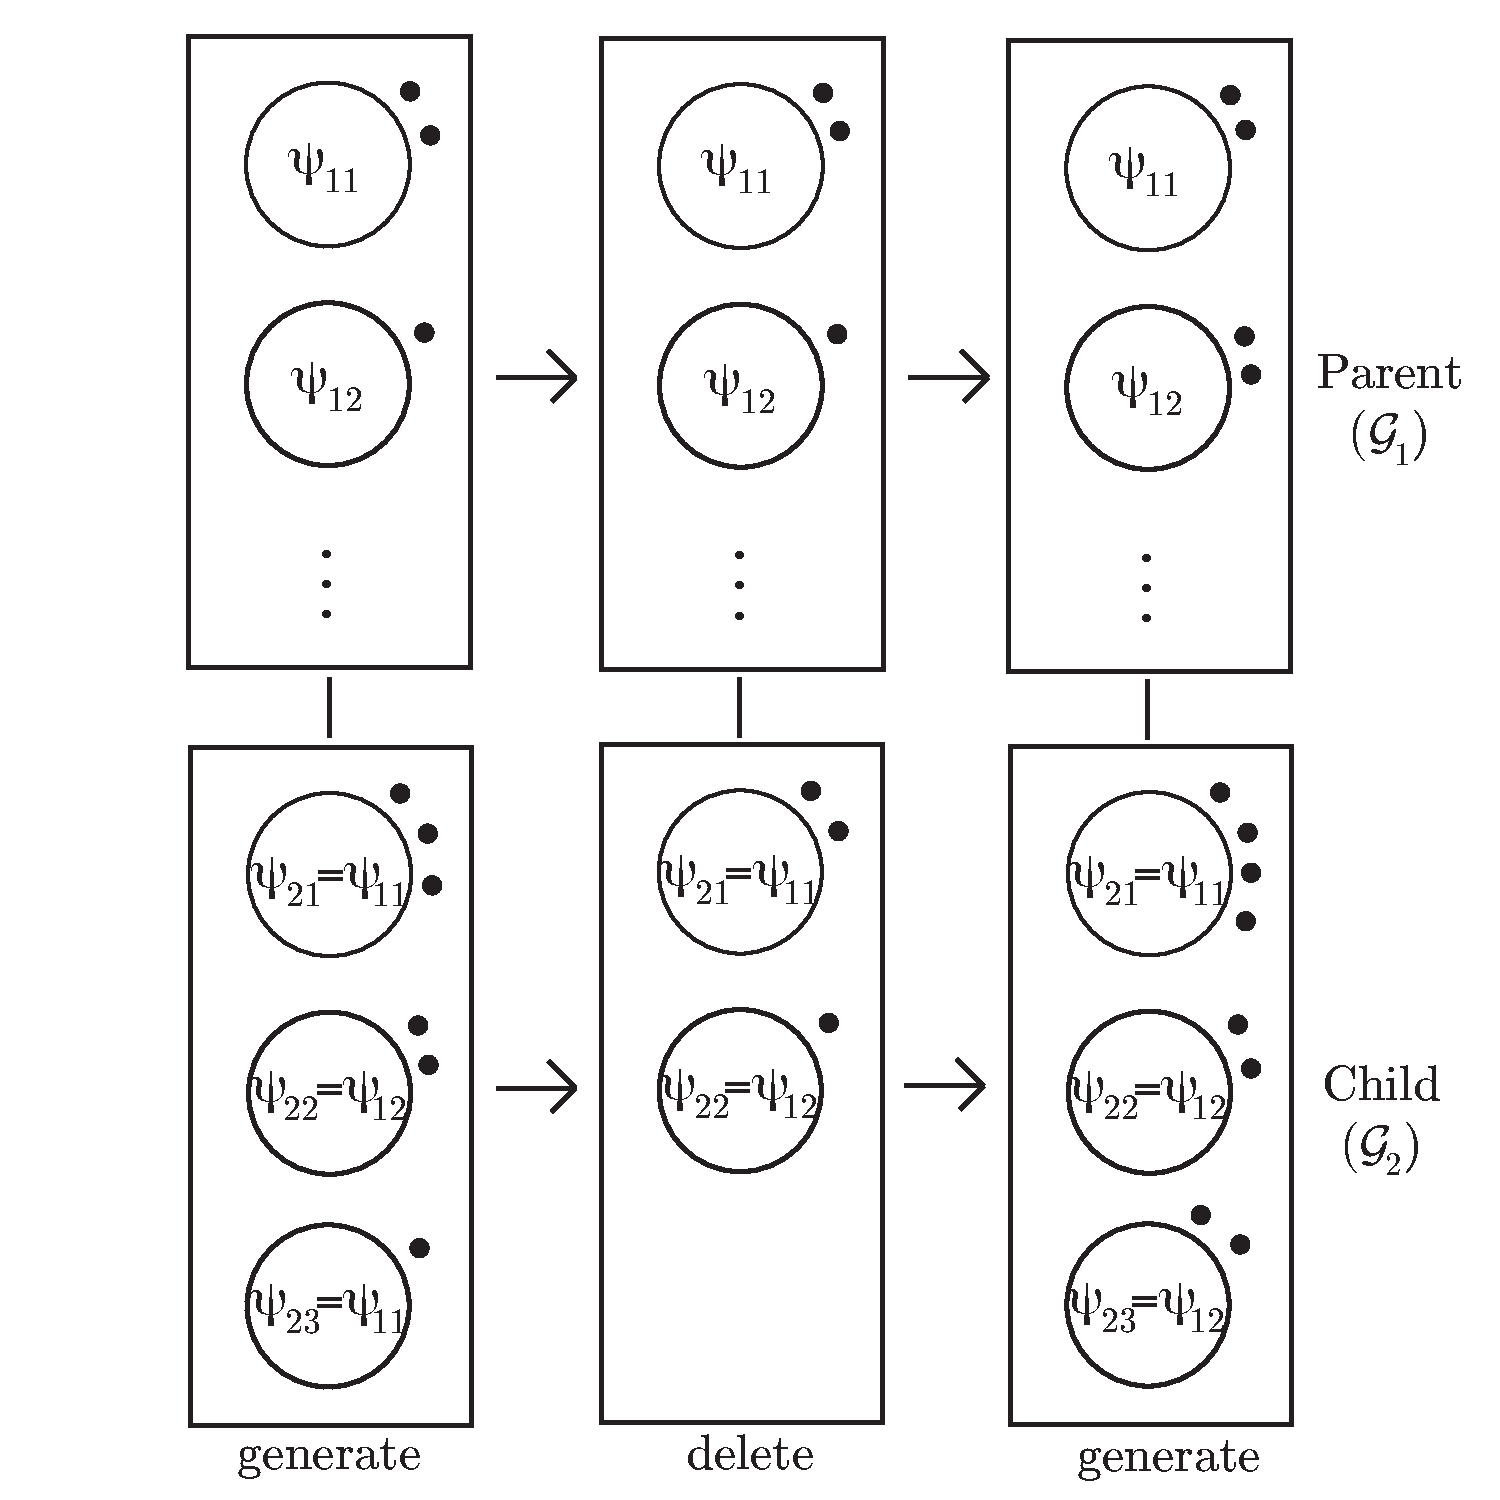
\includegraphics{figure2.pdf}} % [clip=true, viewport= 1in 1in 9in 9in]
		\caption{An example of the possible evolution of the restaurant states in a hierarchical setting}
	\end{center} 
\end{figure} 

Figure~\ref{figVHPY} illustrates the potential evolution of the restaurants used during the CRF process modified to draw a sample from dependent distributions following a Pitman-Yor process distribution.  The middle column of restaurants show the restaurant customer configurations after a deletion step.  Note the configuration of the parent restaurant does not change even though one of the tables in the child restaurant has been removed.  The customer configuration in the third column shows a potential seating arrangement which could have generated the observed sample.  Here, a customer was added to the the parent restaurant in order to generate the parameter $\psi_{12}$  given to the third table in the child restaurant.

Simple extensions allowing for dependent distributions higher on the hierarchy are straightforward.  Given the model specification

\begin{eqnarray*}
\G_1^t | d_1, c_1, \G_0  &\sim& \PY(d_1,d_2,\G_0) \hspace{.5cm} t = 1\dots T\\
\G_2^t | d_2, c_2, \G_1^t &\sim& \PY(d_2, c_2, \G_1^t)  \hspace{.5cm} t = 1\dots T\\
\theta^t_i | \G_2^t &\sim& \G_2^t \hspace{.5cm} i = 1\dots N_t, 
\end{eqnarray*}

if we assume independence of the $\{ \G_2^t \}$ we can use the generalized restaurant procedure to generate samples. The assumption of independence indicates that at each time step the restaurant corresponding to $\G_2$ is emptied of all customers. Without the assumption of independence the extension is not straightforward. Creating a modified restaurant procedure to draw a sample from such a model would require a process to update the customer configuration in the restaurant corresponding to $\G_2$ to reflect changes made to the configuration of the restaurant corresponding to $\G_1$, while maintaining a level of dependence.  It is likely that such a process exists, but it is not necessary for this discussion.

\subsection{Time-varying model applied to SM}

The time-varying model will not only allow for a sequence of time-varying distributions, but can also serve to limit the complexity of the model representation. This framework provides a basis for algorithmic control of the complexity of hierarchical Pitman-Yor models like the SM.  As noted earlier, the number of instantiated restaurants in the SM is the fundamental limiting factor regarding memory usage, thus we will consider a single instantiated restaurant as a unit of memory when discussing the model. For the deletion scheme to limit the amount of memory used by the SM model, we must be able to limit the number of instantiated restaurants.

\begin{figure*}[t] 
	\begin{center}
		\scalebox{.4}{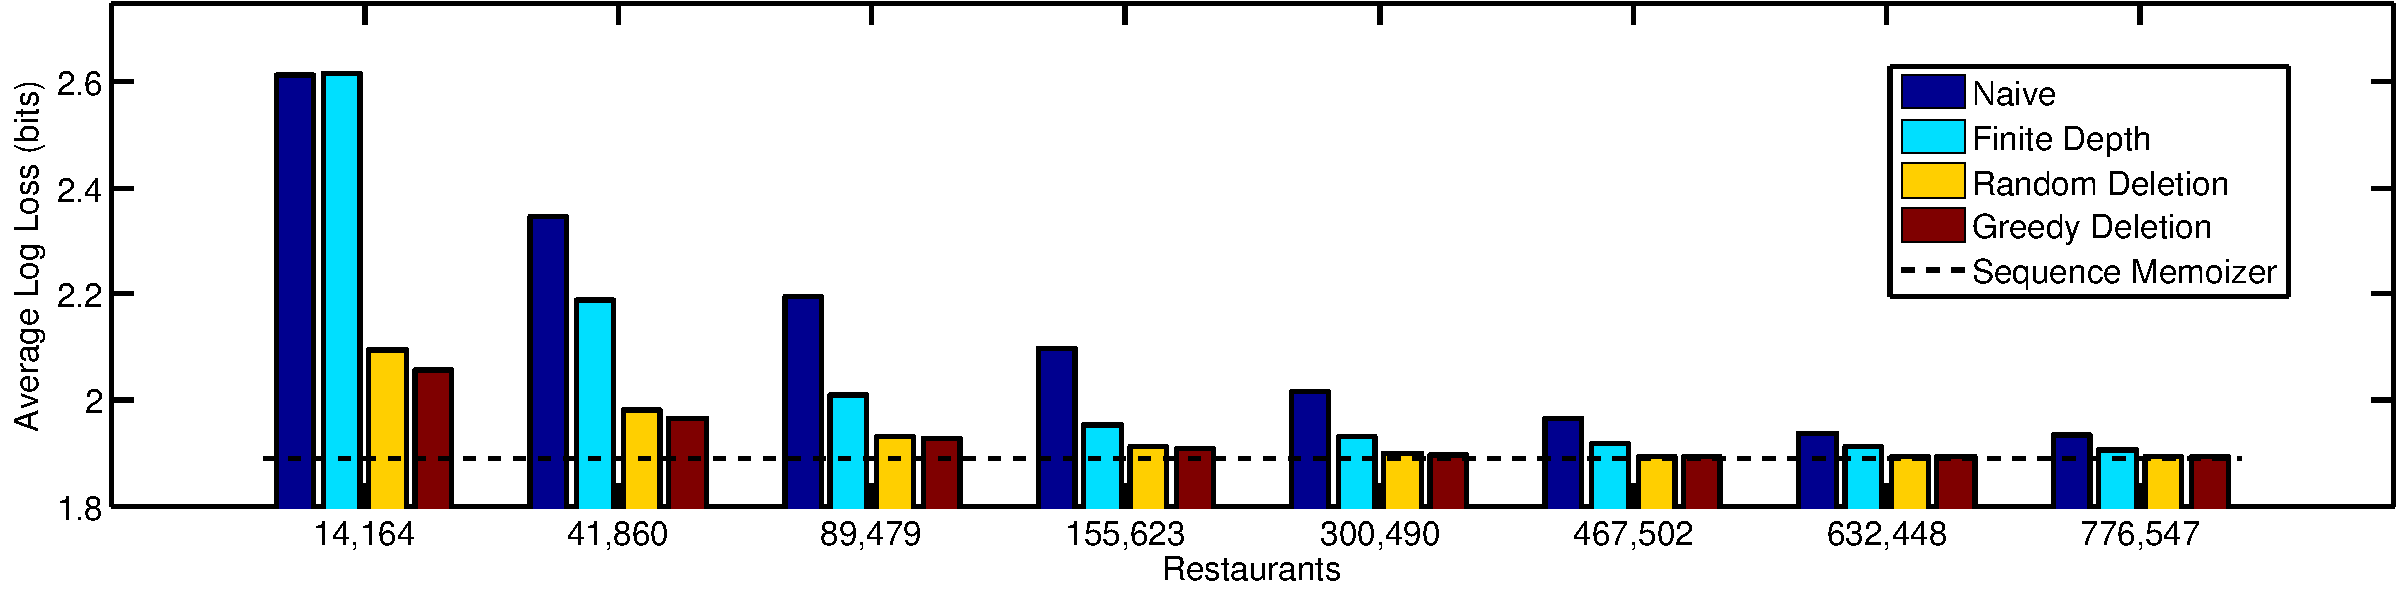
\includegraphics{results_calgary_corpus.pdf}} % [clip=true, viewport= 1in 1in 9in 9in]
		\caption{An example of the possible evolution of the restaurant states in a hierarchical setting}
	\end{center} 
	\label{figResultsCC}
\end{figure*} 

The theory presented above indicates that between time steps we can only delete customers in restaurants at the lowest level.  In the tree which represents the state of the SM, this corresponds to the leaf restaurants.  To achieve memory savings we will need to delete all of the customers at a given restaurant.  Restaurants without people need not be represented in the model state.  This deletion operation gives rise to implicit model assumptions. If, at time step $t$, we delete all the customers in a given leaf restaurant we implicitly assume the distribution over types given the particular context to be independent of the distribution at previous time steps.

It is often the case in the SM model that the parent restaurant for a leaf restaurant is not instantiated, thus to actually attain memory savings by deleting a leaf restaurant we must effectively delete all the restaurants in this particular path up until the nearest instantiated restaurant.  The implicit model assumption is that all of the distributions after time $t$ corresponding to those many deleted restaurants are conditionally independent of their previous states.

This is the basic framework for both bounded memory algorithms we present and is the main contribution of this paper.  The assumption that, for many contexts, the distribution changes over time seems appropriate for very long sequences. The assumption of independence required for us to justify our particular deletion process is primarily of practical motivation though we expect information lost to be minimal. 

Finally, we point out that the theory behind these deletion operations holds for general hierarchical Pitman-Yor processes and thus also for finite depth n-gram style models.  In Section~\ref{results} we show some results concerning this type of model as well.


\section{Inference}
\label{inference}

%The basic model we use is the SM model following the advice of \cite{Gasthaus}.  We parameterize the SM model with a unique discount parameter for each of the first ten depths.  The discount parameter for all depths below ten is set equal to the discount parameter at depth ten.  Furthermore, our generative process specifies that when the number of restaurants reaches a threshold a restaurant is chosen uniformly at random from the set of leaf restaurants and deleted.  Deletion is continued until the number of instantiated restaurants is below the threshold.

Given the motivation for this paper we suggest that inference should be incremental.  An incremental technique known as particle filtering has been explored in several non-parameteric Bayesian settings \cite{Fearnhead2004, others}.  The sequential nature of the generative process we propose makes inference using a particle filter approach straightforward. A particle filter works by using a swarm of particles to approximate the posterior distribution over the model space conditional on observed data.  The approximation is represented as a weighted sample, each particle embodying a possible state of the model.  In view of a new data point the weight of each particle is adjusted to reflect the new information.  In the non-parameteric Bayesian setting, since the parameter space is growing as a function of the length of the data, values for new parameters must be incorporated into each particle.  New parameter values are produced through a proposal distribution which is taken into account when the weight of each particle is updated.  To make the inference more efficient proposal distributions are usually chosen to approximate the posterior distribution of the new parameter given the current set of observed data.

We propose here an inferential procedure for the dependent memory-constrained hierarchical Pitman-Yor process model performed in the modified dependent Chinese restaurant franchise representation.  Using this representation, each observation corresponds to a customer seated in the appropriate restaurant.  The latent parameters in the model are the table at which each customer is seated and the restaurants which are deleted at each deletion step.  For the table assignments, a particle filter in this representation will, for each particle, seat the customer corresponding to the most recently observed data in the appropriate restaurant at a table produced from a proposal distribution.  Since seating a customer may indicate the presence of an additional customer in the parent restaurant, a table for a new customer may need to be proposed in the parent restaurant as well.  It is possible that customers will need to be seated all the way up the path until the restaurant corresponding to the distribution over symbols conditional on an empty context.  The proposal distribution we suggest for choosing a table for each customer is the posterior distribution conditional on the new observation and the current state of the particle.  Details of this inference scheme applied to the SM can be found in \cite{Gasthaus2010}.

When state of the model represented in each particle reaches the memory constraint we will need to propose values for the the latent parameters indicating which restaurants were deleted. We suggest two different proposal distributions to correspond with the two interpretations of the model specification already discussed.  The first is complementary to the understanding of the model as a sequence of dependent distributions with Pitman-Yor process distributions which vary sequentially across the sequence.  The second is complementary to the understanding of the model as a finite state approximation of a model representation which grows linearly as a function of the length of the data.

The first proposal distribution for the deletion of restaurants is uniform over the leaf nodes of the current state of the model.  Using the generative process as the proposal distribution is standard in particle filtering approaches \cite{Doucet2001}.  We refer to the use of this proposal distribution as using a random deletion scheme.

For the second proposal distribution we note that a fixed state of the model represents a likelihood conditional on any context.  We can use this likelihood to approximate the probability of observing the sequence we used to to build the model.  Furthermore, by deleting different leaf restaurants the probability of the sequence, given the updated state of the model, changes and can be approximated in the same way.  The second proposal distribution deterministically proposes the leaf restaurant whose deletion least negatively impacts the likelihood of the observed sequence.  We refer to the use of this proposal distribution as using a greedy deletion scheme. 

While the sequential nature of particle filtering fills the incremental requirement, a particle filter with a large particle swarm could still require too much space.  It is possible to implement particle filtering algorithms where the aspects of the particles which overlap are represented only once and thus induce memory savings.  Using such an algorithm here could be extremely complicated.  We suggest the alternative approach of only using one particle in the particle filter.  This approach was shown to be effective in practice by \cite{Gasthaus201} and simplifies implementation a great deal.


%\subsection{Complexity}

%A little consideration will show that both of the algorithms suggested for inference in this model require constant space, in the sense of the turing machine, and linear time.  The claim that the algorithms are linear in time stems from the fact that each observation must be seated, but now each seating operation is a constant time operation as the length of any path one must traverse in order to seat an observation is bounded by the total number of instantiated restaurants.  Furthermore, each deletion step requires, at worst, visiting every instantiated restaurant, which if done recursively is a constant time algorithm given that the number of instantiated restaurants is limited.  

%The claim that the algorithm requires constant space requires a little more thought.  It is clear that we have limited the space required by restaurant objects, but what about the actual construction of the tree?  Currently our implementation labels each edge between nodes with two integers which index into the original sequence in order to describe that particular edge.  That is, if the parent restaurant corresponds to the distribution over bytes following $oc$,  and the child restaurant corresponds to the distribution over bytes following $acdoc$, the connecting path may be described by the integer array $[17,20]$ if in the sequence being seated, the entries 18-20 are $acd$.  This type of algorithm requires only constant space for each edge, though it works best if the entire sequence is held in memory.  That being said, considering the sequence being seated to be a semi-infinite tape as in the turing machine stipulation, reversals of the tape are allowable.  Thus, the entire sequence need not be held in memory, it is only necessary that we can reverse the tape to access previous entries in the sequence if we need them.

%As a practical side note, an alternative approach to implementation could store the full connecting context on the edge between nodes.  In the above example this would correspond to labeling the edge with the byte array $[acd]$.  While this does not theoretically require constant space, typically when implementing the algorithm on real data only a short section at the end the array is used.  Caching a fixed length section of the each array on the appropriate edge could drastically reduce the number of times the algorithm requires the tape to reverse.  As an example, if one was fitting the entire model on each document of the calgary corpus separately, as we do in the results section, and were willing to cache arrays of length 6,000, a tape reversal would never be required.  This number could only decrease using either of the deletion schemes suggested.  Finally, if we use a fixed depth model, caching the contexts on the edges requires only constant memory when enforcing an upper bound on the number of restaurants.


\section{Experiments and Results}
\label{results}

In tests of predictive probability using incremental inference, the constant space deletion schemes outperformed commercial compressors and simpler constant space models, while approaching the performance of linear space methods even with significantly less space.  The data we used in our experiments was the Calgary Corpus (CC) \cite{Bell1989}.  The CC is a compression benchmark corpus that consists of 14 files chosen to cover a typical range of file types.  A separate instance was trained for every combination of model tested (naive, finite depth, random deletion, greedy deletion) and file.  Files were treated as a sequences of bytes.  Estimation was performed incrementally using Algorithm~\ref{alg1} with $K=1$. The posterior predictive probability of each byte was calculated before that byte was incorporated into the model.  The random number generator was initialized with a new seed for every instance at the start of each run.  Figure~\ref{figResultsCC} shows the average predictive performance of several sequential prediction models (error bars were too small to be included).  The reported results are the per-byte log-loss in bits averaged over all files in the corpus.  \comment{In the compression setting this corresponds directly to compression ratio \cite{Cover1991}.}

%\label{figResultsCC}

To evaluate our two procedures for constant space inference, we compared to the full SM, two other simple constant space versions of the SM and two standard compressors.  The SM does not delete any restaurants and incremental inference is linear in space and time.  The two inference procedures of interest (random and greedy deletion) are both schemes for deleting restaurants from the model, one which randomly deletes restaurants and one which greedily deletes the restaurants which make the smallest change possible to the approximate likelihood of the data already observed, as described in Section~\ref{inference}.  Inference in the naive constant space SM runs the same as for a normal SM until the maximum number of restaurants is reached, at which point all restaurants are removed and inference continues along the remainder of the sequence.  The finite depth model takes the SM and bounds the length of a preceding sequence included in an observation.  Thus, it is a HPYP model with finite tree depth.  Since we cannot know the number of restaurants in a finite depth model before estimation, we perform inference with this model first and use the number of restaurants as an upper bound on the space allowed by the other models, as described below.  We also compressed each file using gzip and bzip2 \cite{Deutsch1996, Seward1999}.  Default parameters were used for the commercial compressors.

\comment{To baseline our model we ran two other constant space sequence models and two standard compressors.  The first was an adaptation of the SM model to finite depths.  By bounding the depth of the SM we create a finite depth HPYP model with concentration parameters zero.  Inference was performed using the single particle particle filter. The second was a naive constant space version of the SM.  Whenever the number of instantiated restaurants in the model reached the threshold a new SM with zero observations was created and used to model the remainder of the sequence, until the memory bound was again reached.  We also compressed each file using gzip and bzip2 \cite{Deutsch1996, Seward1999}.  Default parameters were used for the commercial compressors.}

We first modeled each file with a finite depth SM model and recorded the number of instantiated restaurants.  The model complexity was allowed to grow without bound, meaning the finite depth model was at its full representational capacity.  The maximum number of instantiated restaurants gave an upper bound on the number of restaurants needed to model any file in the corpus with an HPYP model of a given depth.  We calculated this upper bound for depths 2 through 9.  This set of bounds was then used as the maximum number of restaurants for the naive model and the random and greedy deletion models.  Results are listed in Figure~\ref{figResultsCC}.  For comparison, the full SM model instantiated 1,160,765 restaurants when trained on the same documents.  

Each of the four sequence models were fit ten times.  From that the variance of the inference procedure was estimated.  Our results show the standard deviation of the average log loss to be less than $0.002$ for all of the methods.  All differences detectable in the graph are significant at the $\alpha = 0.01$ level. We note that the SM model paired with either deletion scheme consistently outperforms the finite depth model and the naive model.  We also note that both deletion schemes approach quite close to the performance of the full SM with only one sixth as many restaurants.  Furthermore, the greedy deletion scheme shows improvement over the random deletion scheme, especially for low thresholds.  The SM model paired with either deletion scheme outperformed the commercial compressors at every threshold tested.


\section{Discussion}
\label{discussion}



\bibliography{../../uber.bib}
\bibliographystyle{icml2010}

\end{document} 
